%\documentclass{article} % For LaTeX2e
\documentclass[answers]{exam}
\usepackage{cos424,times}
\usepackage{hyperref}
\usepackage{url}
\usepackage{graphicx}
\usepackage{enumitem}
\usepackage{wrapfig}
% For LaTeX2e
\usepackage{cos424,times}
\usepackage{hyperref}
\usepackage{url}
\usepackage{graphicx}
\usepackage{wrapfig}
\usepackage{amsmath}
\usepackage{enumitem}
\usepackage{booktabs}
% packages that allow mathematical formatting
\usepackage{setspace}
% package that allows you to change spacing
\usepackage{comment}
% text become 1.5 spaced

\usepackage{fullpage}
% package that specifies normal margins
\usepackage{amsmath}
\usepackage{graphicx}
\usepackage{float}
\usepackage{listings}
\usepackage{subfig}
\usepackage{bbm}
\usepackage{multirow}
\usepackage{booktabs}

\title{CME Homework Assignment 3 Computational Work}


\author{
Jacob Perricone \\
Stanford University\\
\texttt{jacobp2@stanford.edu} \\, \and
\textbf{Ian Shaw}\\
Stanford University\\
\texttt{ieshaw@stanford.edu} \\, \and
\textbf{Weronika \`Swi\c echowicz} \\ 
Stanford University\\
\texttt{wswiecho@stanford.edu}
}




\newcommand{\fix}{\marginpar{FIX}}
\usepackage{xcolor}
%\usepackage{mathbb}
\usepackage{sympytex}
\usepackage{color}
\usepackage{sectsty}
\sectionfont{\LARGE\underline}
\subsectionfont{\underline\normalsize}
\subsubsectionfont{\underline\normalsize\itshape}


\definecolor{mygreen}{rgb}{0,0.6,0}
\definecolor{mygray}{rgb}{0.5,0.5,0.5}
\definecolor{mymauve}{rgb}{0.58,0,0.82}

\lstset{ %
backgroundcolor=\color{white},   % choose the background color; you must add \usepackage{color} or \usepackage{xcolor}
basicstyle=\footnotesize,
flexiblecolumns=true      % the size of the fonts that are used for the code
breakatwhitespace=false,         % sets if automatic breaks should only happen at whitespace
breaklines=true,                 % sets automatic line breaking
captionpos=b,                    % sets the caption-position to bottom
commentstyle=\color{mygreen},    % comment style
deletekeywords={...},            % if you want to delete keywords from the given language
    escapeinside={\%*}{*)},          % if you want to add LaTeX within your code
    extendedchars=true,              % lets you use non-ASCII characters; for 8-bits encodings only, does not work with UTF-8
    frame=single,                    % adds a frame around the code
    keepspaces=true,                 % keeps spaces in text, useful for keeping indentation of code (possibly needs columns=flexible)
    keywordstyle=\color{blue},       % keyword style
    language=Matlab,                 % the language of the code
    otherkeywords={*,...},           % if you want to add more keywords to the set
    numbers=left,                    % where to put the line-numbers; possible values are (none, left, right)
    numbersep=5pt,                   % how far the line-numbers are from the code
    numberstyle=\tiny\color{mygray}, % the style that is used for the line-numbers
    %rulecolor=\color{black},         % if not set, the frame-color may be changed on line-breaks within not-black text (e.g. comments (green here))
    showspaces=false,                % show spaces everywhere adding particular underscores; it overrides 'showstringspaces'
    showstringspaces=false,          % underline spaces within strings only
    showtabs=false,                  % show tabs within strings adding particular underscores
    stepnumber=2,                    % the step between two line-numbers. If it's 1, each line will be numbered
    stringstyle=\color{mymauve},     % string literal style
    tabsize=2,                     % sets default tabsize to 2 spaces
    title=\lstname,
    % Single frame around code                               % show the filename of files included with \lstinputlisting; also try caption instead of title
    }
    
    \newcommand{\E}{{\mbox {\bf E}}}
    \newcommand{\me}{\mathrm{e}}
    \newcommand{\I}{\mathbbm{1}}
    \newcommand{\R}{\mathbbm{R}}
    \newcommand{\Q}{\mathbbm{Q}}
    \newcommand{\Z}{\mathbb{Z}}
    \newcommand{\N}{\operatorname{N}}
    \newcommand{\C}{\operatorname{C}}
    \newcommand{\f}[1][]{\hat{#1}}
    \newcommand{\rev}[1]{\frac{1}{#1}}
    % \newcommand{+binomial}[3][2]{(#2 + #3)^#1}
    \newcommand{\prev}[1]{#1_{t-1}}
    \newcommand{\nex}[1]{#1_{t+1}}
    \newcommand{\now}[1]{#1_t}
    \newcommand{\ttwo}[1]{\now{#1}^{2}}
    \newcommand*{\dprime}{^{\prime\prime}\mkern-1.2mu}
    \newcommand*{\tprime}{^{\prime\prime\prime}\mkern-1.2mu}
    
    \newcommand{\ptwo}[1]{\prev{#1^{2}}}
    \newcommand{\h}[1]{\expandafter\hat#1}
    \newcommand{\ti}[1]{\widetilde{#1}}
    \newcommand{\B}[1]{\mathbf#1}
    \newcommand{\ii}[1]{\mathit#1}
    \newcommand{\that}[1]{\mathbf{\hat{#1}}}
    \newcommand{\ttil}[1]{\mathbf{\tilde{#1}}}
    \newcommand{\new}{\marginpar{NEW}}
    %\usepackage[active]{srcltx}
%\usepackage{fullpage}
%\usepackage[dvips]{graphicx}
%\DeclareGraphicsExtensions{.eps} \graphicspath{{images/}}
\linespread{1.3}
\parskip 1ex  \parindent 0ex
%\voffset -15mm
\oddsidemargin -0mm \topmargin 0mm \headheight 0pt \headsep 0pt
\textwidth 6.5in \textheight 9in %\marginparsep 0pt \marginparwidth 0pt
\renewcommand{\baselinestretch}{1.3}
\newtheorem{prop}{Proposition}
\newtheorem{Cor}{Corollary}
\newtheorem{lema}{Lemma}
\renewcommand\a{{\bf a}}
\renewcommand\b{{\bf b}}
\newcommand\x{{\bf x}}
\newcommand\s{{\bf s}}



\def \NATUR{ I \hspace*{-0.8ex} N}
\def \REALES{ I \hspace*{-0.8ex} R}
\renewcommand{\labelenumi}{\alph{enumi})}
\renewcommand{\labelenumii}{\roman{enumii})}


\begin{document}
\maketitle

    
\section*{Problem 2.d } (Computation Team Work) Apply any Quasi-Newton (e.g., slide 18 of Lecture \#13 or L\&Y Chapter 10) and Newton methods to solve the problem using the data in HW2 for SVM (may or may not with regulation), randomly generate data sets, and/or benchmark data sets you can find. Compare the two methods with each other and with the previous methods used in HW3.


\newpage
\begin{framed}


Using the dataset from last week and scrapping the regularization component, let us compare the different methods:


Both the Newton Method an the DFP method appear to enjoy fast convergence rates. An $\alpha$ of one was chosen for Newton Method, whereas for the DFP method, $\alpha_k$ was chosen to minimize the objective function in the direction of $d = - H_k g_k$. 
    
    \begin{figure}[H]
    \centering
    \caption{Convergence Of Second Order Method}
    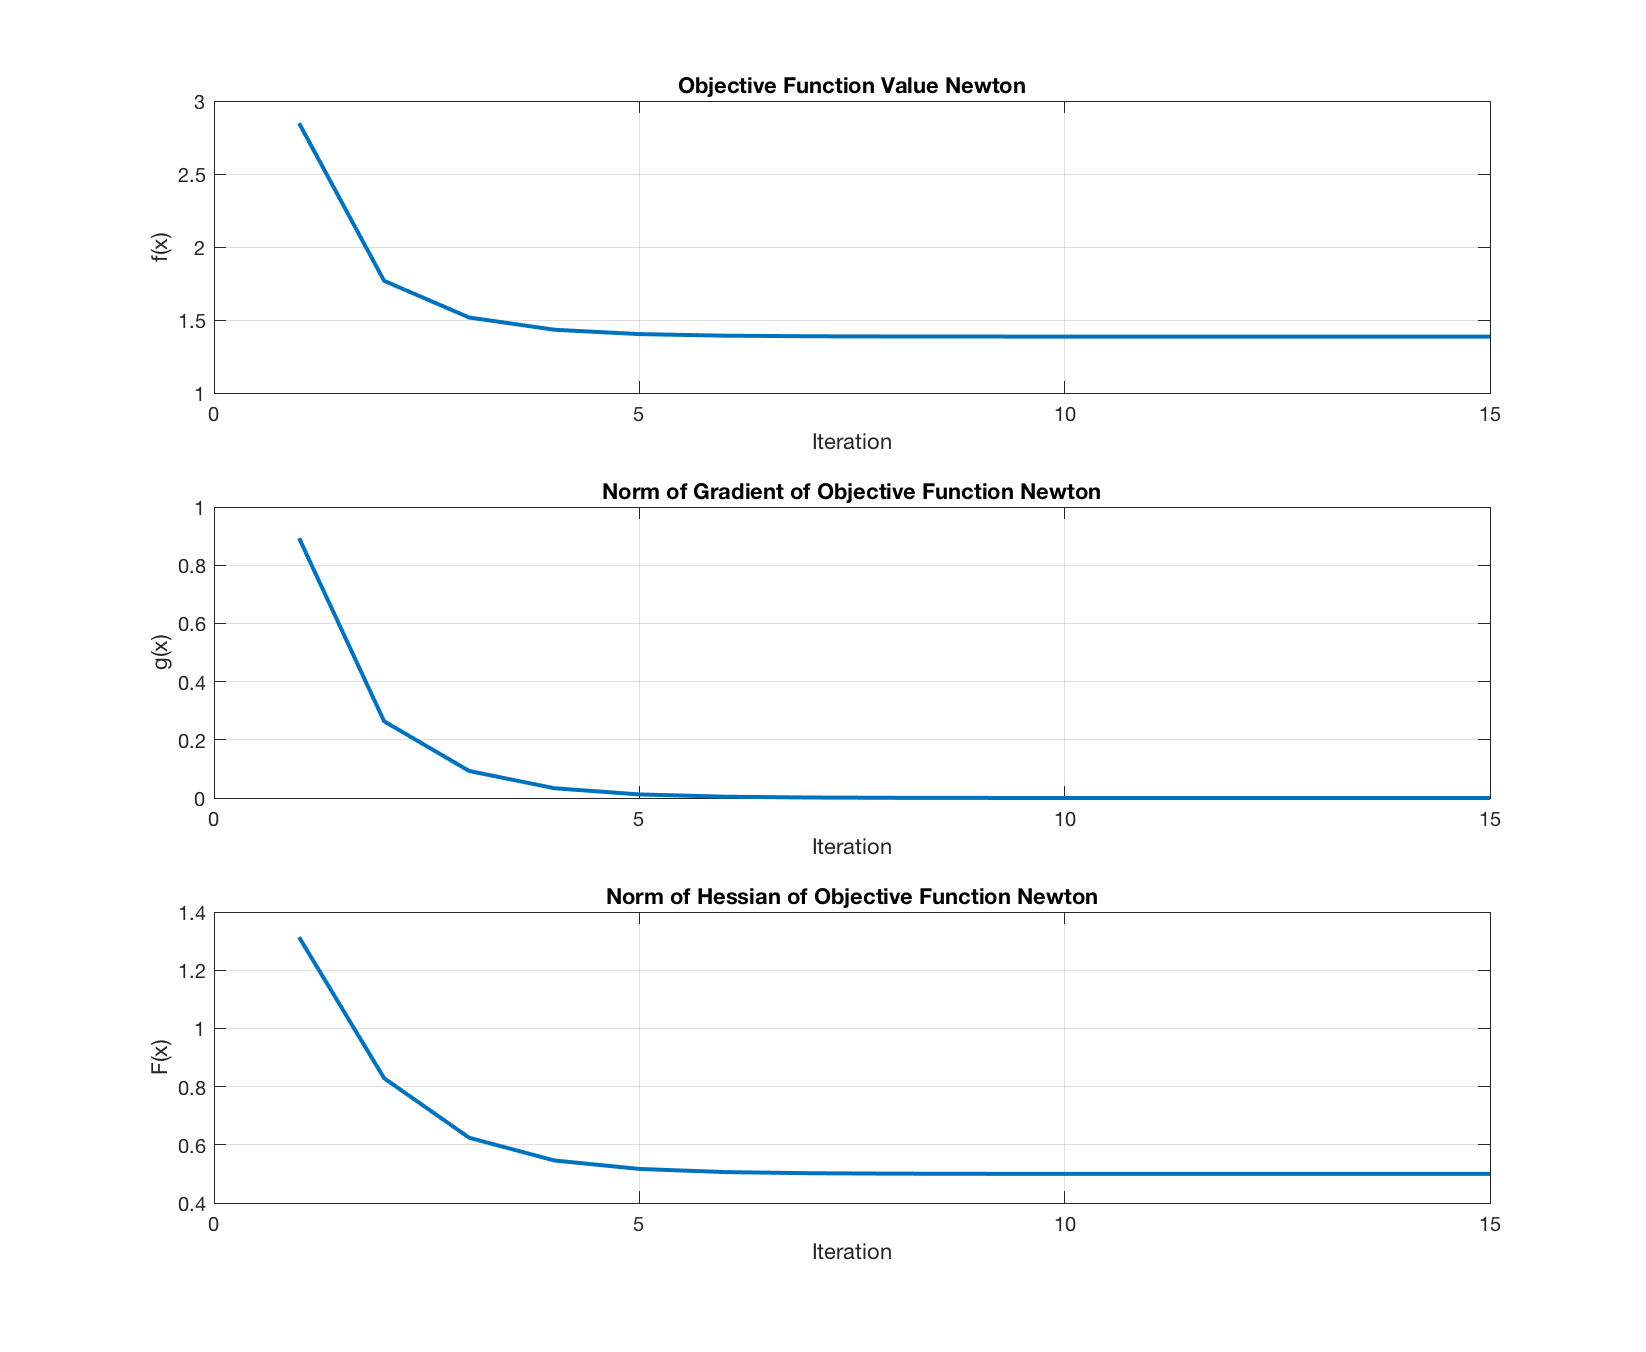
\includegraphics[width=\linewidth, height=9cm]{NEWTON_PLOT.png}
    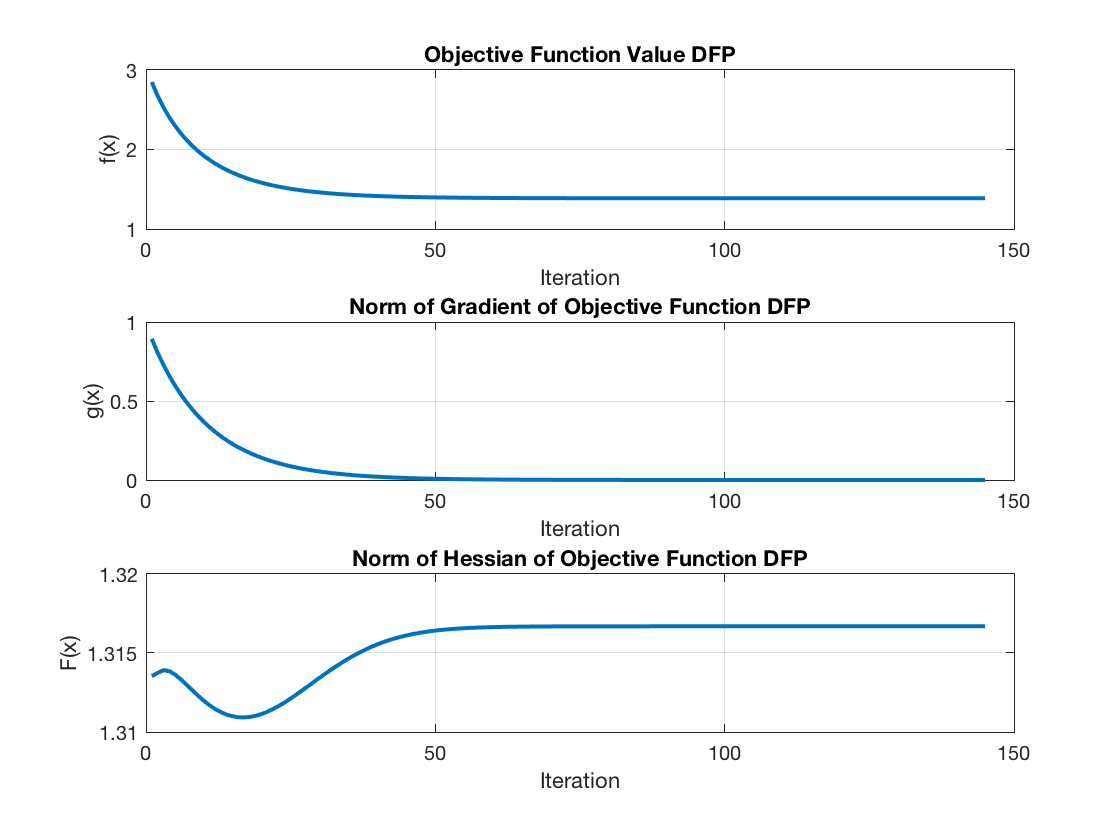
\includegraphics[width=\linewidth, height=9cm]{DFP_PLOT.png}
    \end{figure} 

    
    
    Newton's Method Appears to converge more quickly than the DFP method, converging after only $15$ iterations. The DFP method, on the other hand, converges after $145$ iterations, which relative to the methods last week, is very quick. I believe that it is possible to speed up the DFP method if one changes the initial $\alpha$ passed into the line search routine. Essentially, the line search just halves $\alpha$ if the $f(x + \alpha_k H_k d_k) \geq f(x)$. Indeed, if I begin the search with an alpha of $1$ the DFP converges after only $30$ iterations, whereas if I start with an alpha of $.1$ the DFP method takes $145$ iterations. THe plot below overlays the convergence of the two methods in logspace. 

    
     \begin{figure}[H]
    \centering
    \caption{Convergence Comparison}
    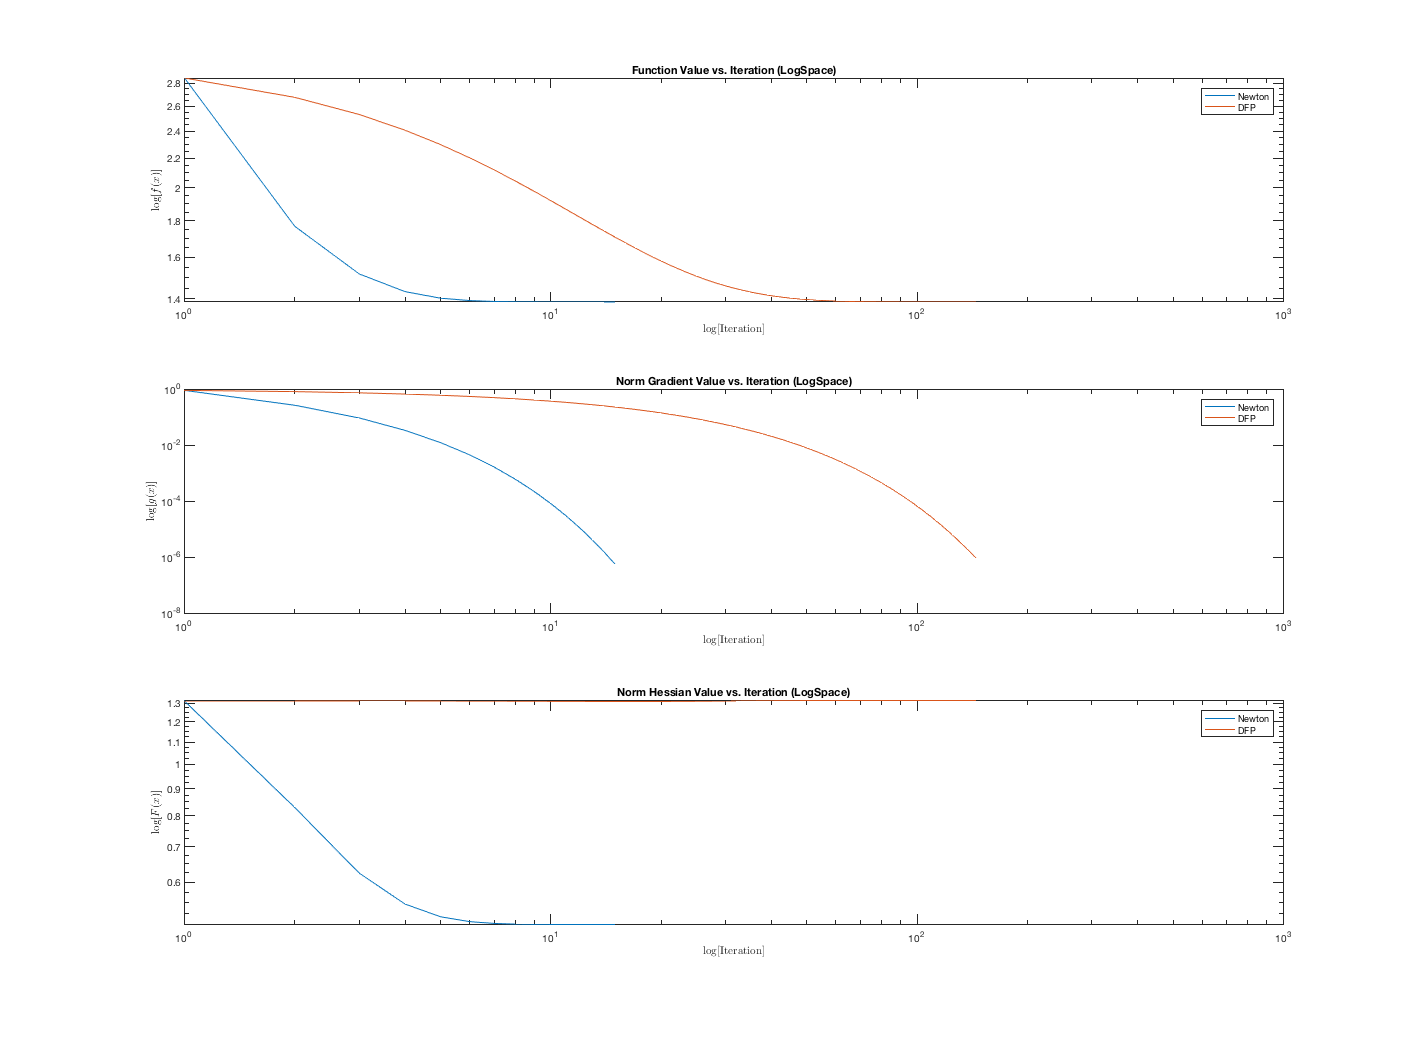
\includegraphics[width=\linewidth, height=15cm]{Problem2_Newton.png}
    \end{figure} 
    
    
    Notice how the norm of the hessian for the DFP method does not decrease with iteration. This is attributed to the fact that it locally approximates the Hessian instead of actually computing it. 
    
    Now let us examine the convergence of the second order methods with respect to the first order methods of last homework. 
    \begin{figure}[H]
    \centering
        \caption{Convergence  Of All Methods}
    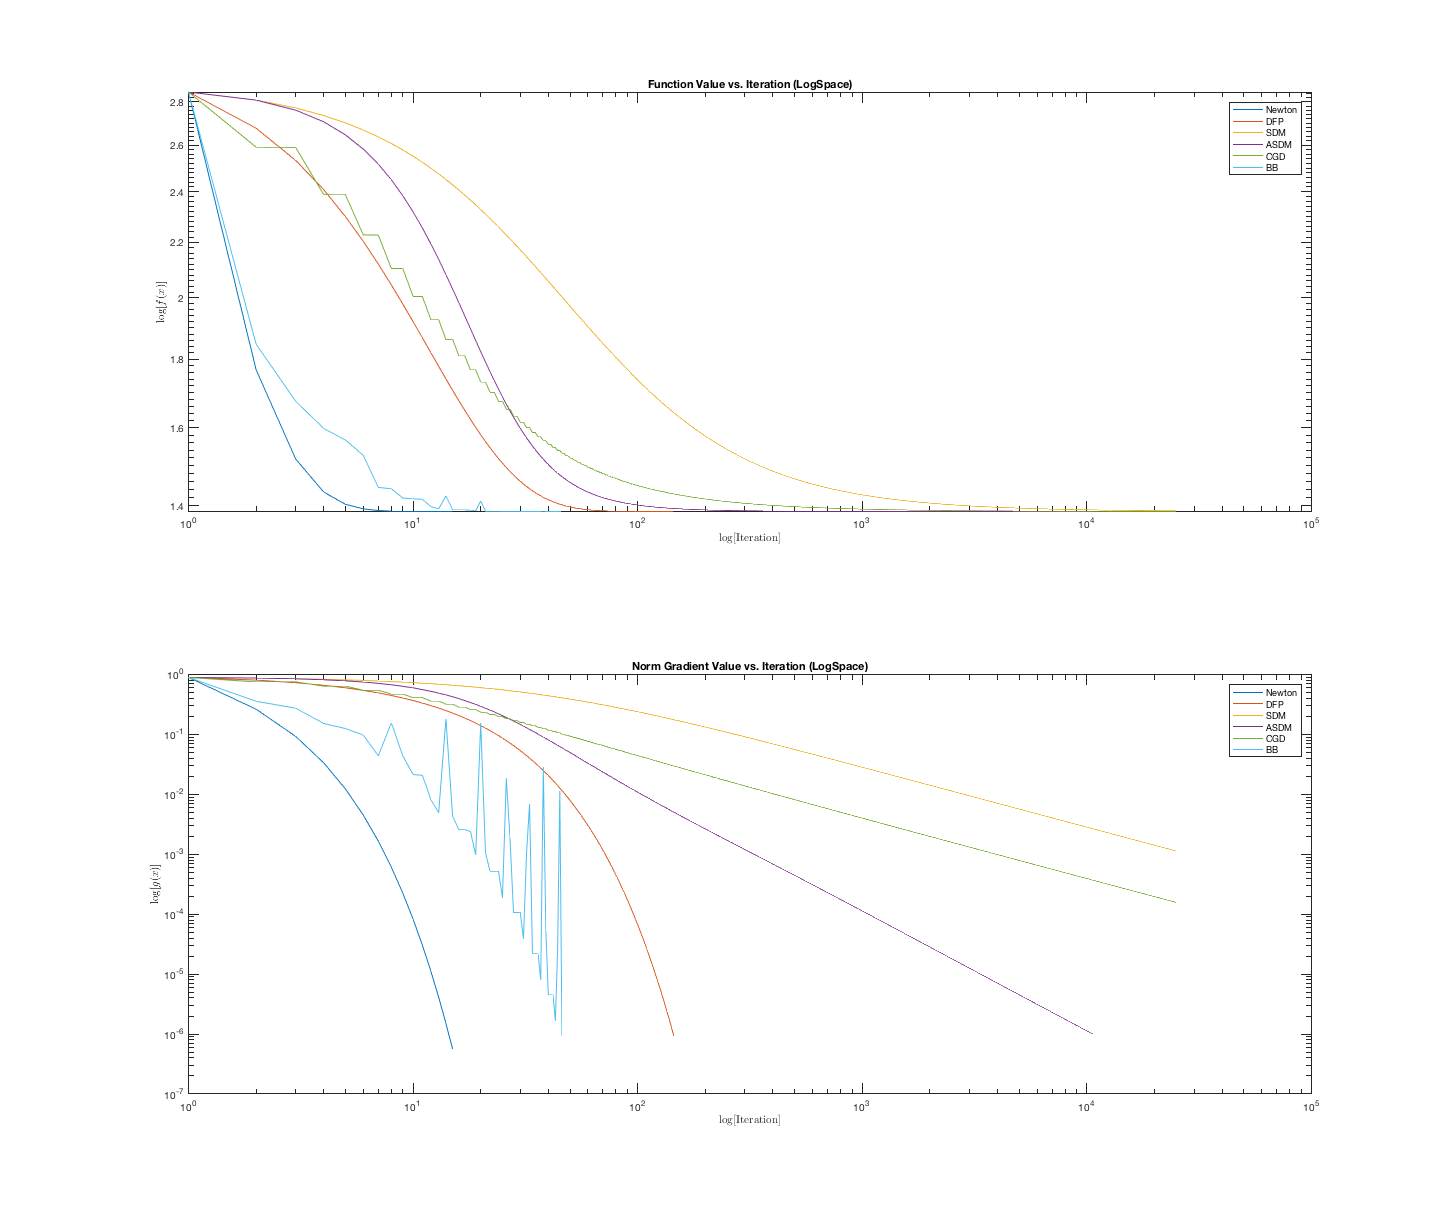
\includegraphics[width=\linewidth, height=18cm]{Problem2_TOGETHER.png}
    \end{figure} 
    
Newton's Method converges the most quickly followed by the Barzilai-Borwein Method, the DFP Method, the CGDM, and the stepest decent methods. The BB method works well with $\alpha_k = \frac{(\nabla_x^k)^{\top} \nabla_g^{k}}{(\nabla_g^{k})^{\top} \nabla_g^{k}}$, but is less appealing than the Newton or DFP methods due to the volatility of its gradient values. This is due to the fact that the stepsize is based on an approximation of the second derivative which can change largely per iteration. Overall, the second order method's have far superior performance than the first order methods. 
    

    
\end{framed}
\newpage

\subsection*{Problem 3.d }
(Computation Team Work) Draw $\x$ part of the primal-dual potential function level sets:
\[\psi_{6}(\x,\s)\le 0 \quad\mbox{and}\quad \psi_{6}(\x,\s)\le -10,\]
and
\[\psi_{12}(\x,\s)\le 0 \quad\mbox{and}\quad \psi_{12}(\x,\s)\le -10;\]
respectively in the primal feasible region (on a plane).

{\bf Hint:} Sample interior points in the primal and dual feasible regions.To plot the $\x$ part of the level set of potential function, say $\psi_{6}(\x,\s)\le 0$,
in primal feasible region $F_p$, you plot
\[\{\x\in F_p:\ \min_{\s\in F_d}\psi_{6}(\x,\s)\le 0\}\]
where $F_d$ represents the dual feasible region. This can be approximately done by sampling as follows.

You randomly generate $N$ interior feasible points of the primal $\x^p$ and the dual $(y^q,\s^q)$, respectively. For 
each primal point $\x^p$, you find if it is true that
\[\min_{q=1,...,N}\psi_{6}(\x^p,\s^q)\le 0.\]
Then, you plot those $\x^p$ who give an "yes" answer.

\begin{framed}
For the plot of the level set $\phi_6(\x,\s)$, even with 10,000 points generated, not points fall within the level set paramaterized by $\phi(\x,\s) \leq -10$. 
    \begin{figure}[H]
    \centering
    \caption{ $\phi_6(\x, \s), f(x) = x_1 + x_2$}
    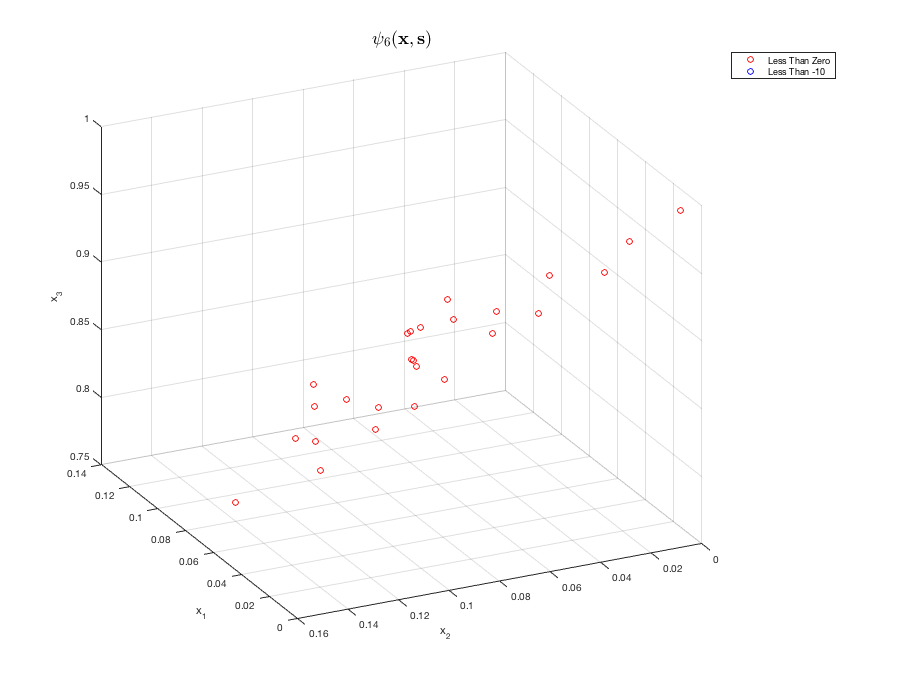
\includegraphics[width=\linewidth, height=8cm]{TF6.png}
    \end{figure}

\newpage
With $\phi_{12}(\x,\s)$ a smaller number of points near $(0,0,1)$-- which is the none optimal solution, have a potential of less than -10. This is as expected, since as you decrease the level set of the potential, the duality gap decreases, indicating an optimal solution. 
    \begin{figure}[H]
    \centering
    \caption{ $\phi_{12}(\x, \s), f(x) = x_1 + x_2$}
    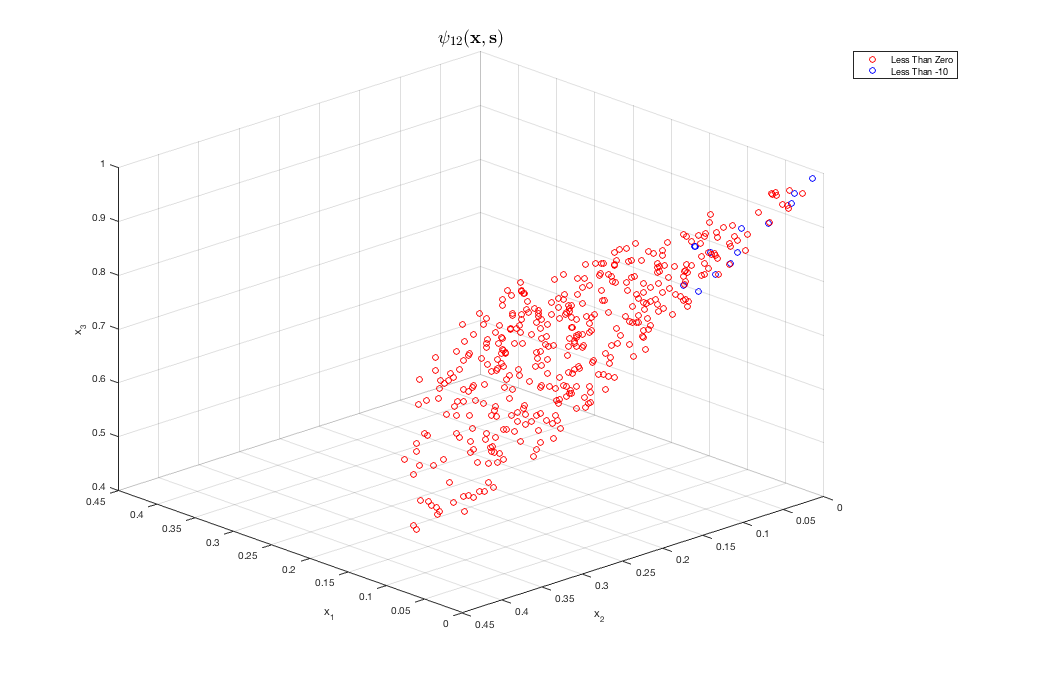
\includegraphics[width=\linewidth, height=8cm]{TF12.png}
    \end{figure} 
    
    
In the case where the objective $f(x) = x_1$, the optimal solution is given by $(0,\frac{1}{2},\frac{1}{2})$. Similar to above, the level set of $\phi_6(\x,\s)$ has very few points with potential less than $-10$, with the only blue point appearing around $(0,.4,.6)$.  

    \begin{figure}[H]
    \centering
    \caption{ $\phi_6(\x, \s),  f(x) = x_1$}
    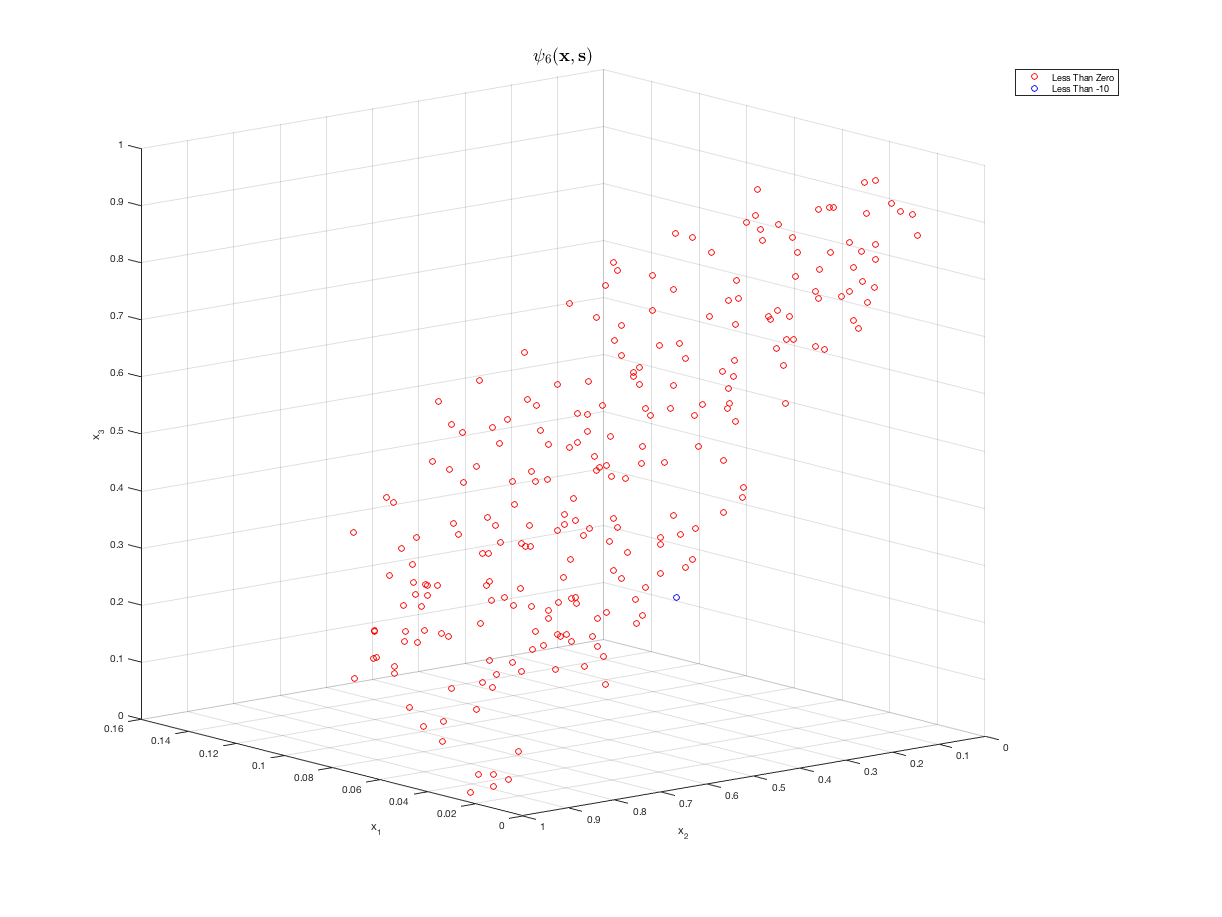
\includegraphics[width=\linewidth, height=8cm]{TF6_2.png}
    \end{figure} 
    
In the case of $\phi_{12}(\x,\s)$, we have many more points with potential less than $-10$, most of which are clustered around $x_1 = 0$. The largest concentration appears in the region $(0, [.4,.6], [.4,.6])$ indicating that decreasing the potential indeed decreases the duality gap. However, there is a large number of points spread along the $x_2, x_3$ plane, suggesting a lower potential set is needed to shorten the duality gap. In fact, if one parameterizes the level set $\phi_{12}(\x,\s) \leq -45$, the only blue point appears at $x_1 = 0, x_2 = .47, x_3 = .53$, which is close to the opimum  
        \begin{figure}[H]
    \centering
        \caption{ $\phi_{12}(\x, \s), f(x) = x_1$}
    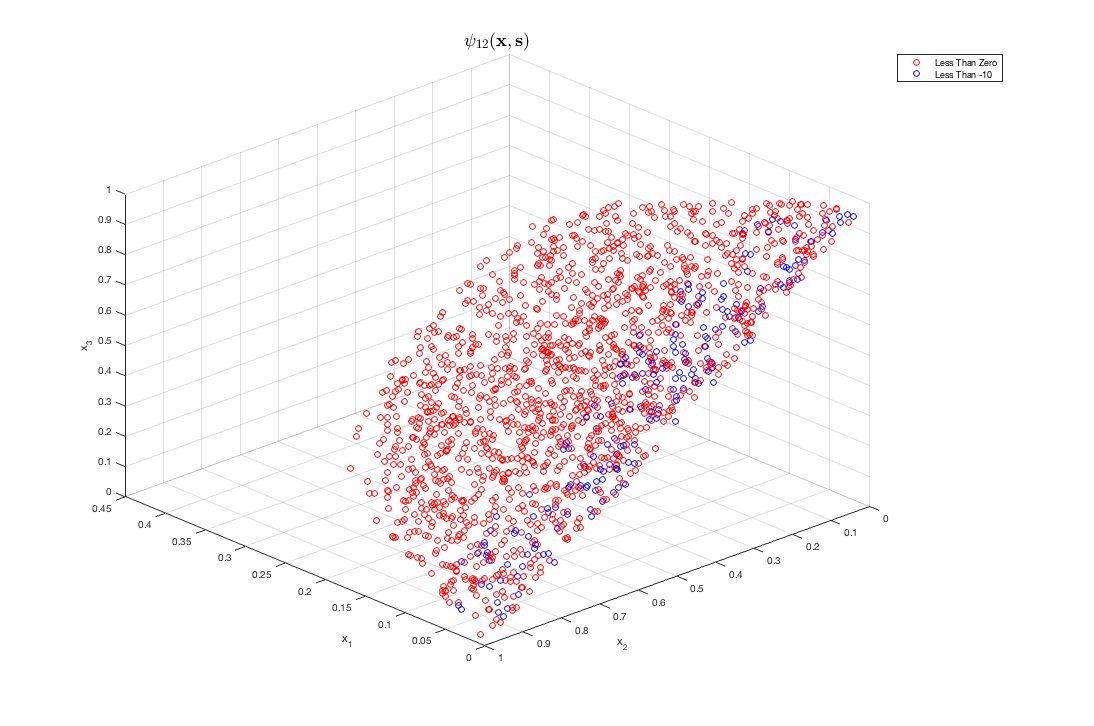
\includegraphics[width=\linewidth, height=8cm]{TF12_2.png}
\end{figure}

\end{framed}
\subsection*{Problem 7} Implement the ADMM to solve the divergence example in Lecture \&16.
\begin{itemize}
\item[(a)] Try $\beta=0.1$, $\beta=1$, and $\beta=10$, respectively. Does the choice of $\beta$ make a difference? 

\begin{framed}
By studying left plots in figures 11-13, it should be clear that the ADMM fails to find a convergent solution to the given problem independently of the value of $\beta$. The only difference we can observe in these graphs is the magnitude of oscillation from the true value of $x$, which decreases with the increases in the value of $\beta$.
\end{framed}
\newpage
\item[(b)] Add the objective function to minimize
\[0.5(x^2_1+x^2_2+x^2_3)\]
to the problem, and retry $\beta=0.1$, $\beta=1$, and $\beta=10$, respectively. Does the choice of $\beta$ make a difference?

\begin{framed}
The right hand side plots in figures 11-13 depict the convergence/divergence of the estimated value of $x$ for different values of $\beta$ when objective function is introduced to the general problem. It should be clear that the ADMM now fails to find a convergent solution only for $\beta=10$. The estimation, however, converges for $\beta=0.1$ and $\beta=1$.
\begin{figure}[H]
    \centering
    \caption{Convergence of $x$ for fixed value of $\beta=0.1$.}
    \begin{minipage}{.5\textwidth}
        \centering
        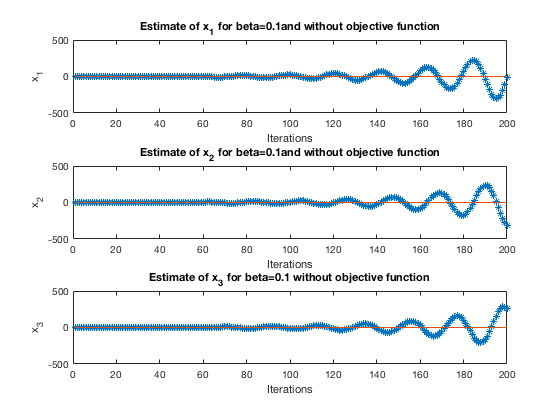
\includegraphics[width=\textwidth, height=0.45\textheight]{Problem7_1.png}
    \end{minipage}%
    \begin{minipage}{0.5\textwidth}
        \centering
        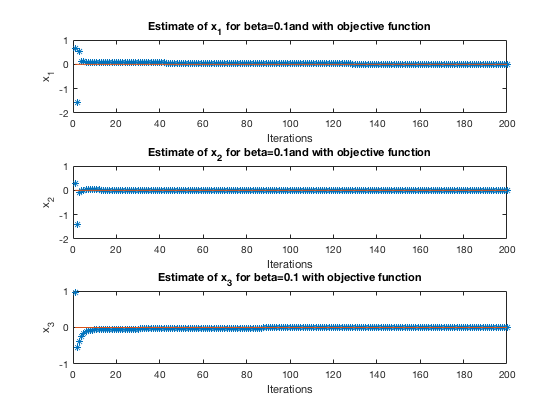
\includegraphics[width=\textwidth, height=0.45\textheight]{Problem7_2.png}
    \end{minipage}
    \label{ob01}
\end{figure}
From the above plots (Fig.~\ref{ob01}), it should be clear that the ADMM fails to find a convergent solution when we optimize the divergent problem without the objective function. However, when the objective function is introduced, it follows that the ADMM converges in less than 100 iterations. 

\begin{figure}[H]
    \centering
    \caption{Convergence of $x$ for fixed value of $\beta=0.1$.}
    \begin{minipage}{.5\textwidth}
        \centering
        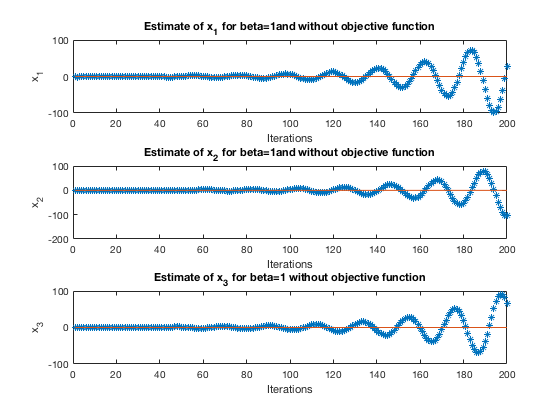
\includegraphics[width=1.1\textwidth, height=0.4\textheight]{Problem7_3.png}
    \end{minipage}%
    \begin{minipage}{0.5\textwidth}
        \centering
        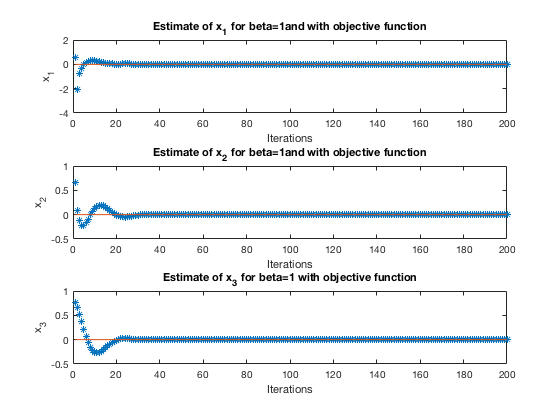
\includegraphics[width=1.1\textwidth, height=0.4\textheight]{Problem7_4.png}
    \end{minipage}
    \label{ob1}
\end{figure}
From the plots in Fig.~\ref{ob1}, it should be clear that the ADMM fails to find a convergent solution when we optimize the divergent problem without the objective function. However, when the objective function is introduced, it follows that the ADMM converges in less than 40 iterations. If we observe the difference between Fig.~\ref{ob01} and Fig.~\ref{ob1}, we notice that for a larger value of $\beta$ the ADMM converges with a smaller number of iterations. Similarly, when the ADMM is applied to a divergent problem with no objective function, the magnitude of divergence from the real soltuion is smaller for greater value of $\beta$, in this case for $\beta=1$.
\begin{figure}[H]
    \centering
    \caption{Convergence of $x$ for fixed value of $\beta=10$.}
    \begin{minipage}{.5\textwidth}
        \centering
        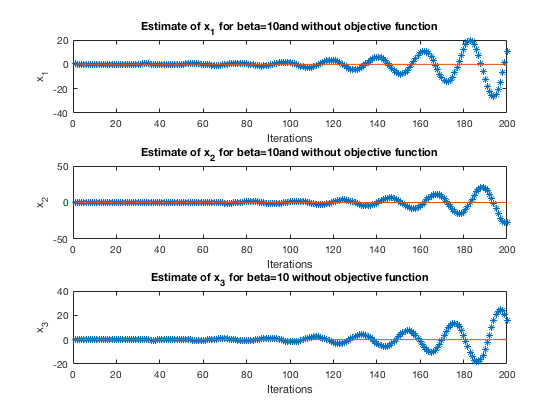
\includegraphics[width=1.1\textwidth, height=0.3\textheight]{Problem7_11.png}
    \end{minipage}%
    \begin{minipage}{0.5\textwidth}
        \centering
        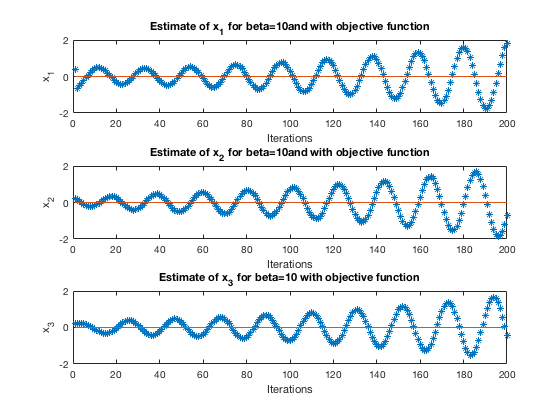
\includegraphics[width=1.1\textwidth, height=0.3\textheight]{Problem7_22.png}
    \end{minipage}
    \label{ob10}
\end{figure}
Fig.~\ref{ob10} shows that the ADMM method fails to find a convergent solution with and without the objective function. That may suggest that when $\beta$ is too large the objective function cannot regularize the optimization problem which will continue to grow without a bound. It addition, the ADMM estimator without the objective function has a smaller magnitude of oscillation from the true value of $x$ than the ADMM estimator with the addition of the objective $f(x)$.


\begin{figure}[H]
    \centering
    \caption{$||Ax||$ for all Methods.}
    \begin{minipage}{.5\textwidth}
        \centering
        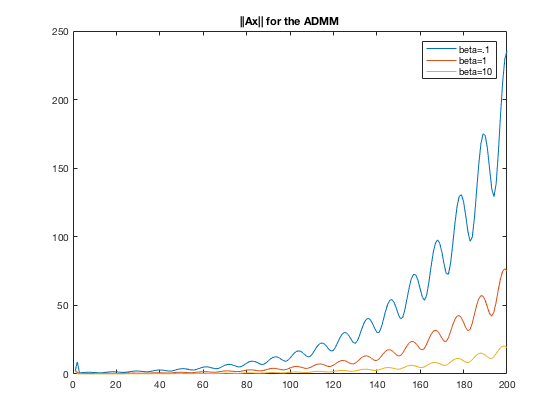
\includegraphics[width=1.1\textwidth, height=0.3\textheight]{Problem7_3a.png}
    \end{minipage}%
    \begin{minipage}{0.5\textwidth}
        \centering
        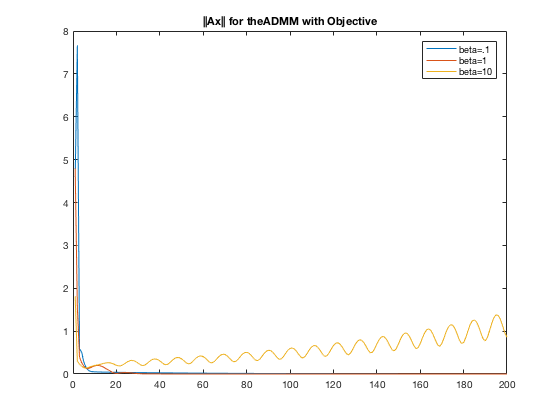
\includegraphics[width=1.1\textwidth, height=0.3\textheight]{Problem7_4a.png}
    \end{minipage}
    \label{normADMM}
\end{figure}
Fig.~\ref{normADMM} shows the norm of the product of a matrix $A$  and a solution of the problem $x$. As it can be easily seen from the plot the left, the ADMM fails to find the optimal solution that converges and thus the norm grows periodical without a bound. That growth is independent of the value of $\beta$, as well as the initial guess for $x$, as long as $x_0\not=0$. The plot on the right, on the other hand, shows that when $\beta\not=10$ (norm diverges for $\beta=10$), the ADMM supported with the objective function finds the true solution of the divergent problem. Thus, for $\beta=0.1$ and $\beta=1$, the norm converges to 0, as the true solution of $x=0$. 
~\\
\end{framed}
\newpage
\item[(c)] Set $\beta=1$ and apply the random permutation updating order of $\x$ (discussed in class) to solving each of the two problems in (a) and (b). Does the iterate converge? 
~\\
~\\

\begin{framed}
Based on Fig.~\ref{p01}-\ref{p10}, it should be clear that the ADMM with permutation finds a convergent solution that equals the true solution of for the given problem. We see that the method converges for all values of $\beta$ not only $\beta=1$. That implies that the introduction of random updating of $x_i$ with $i=\{1,2,3\}$ prevents the solution from growing without a bound. In addition, the mentioned graphs show that the ADMM with permutation converges in a smaller number (approximately 20 vs. 200) of iterations when the objective function is added to the original problem. 



\begin{figure}[H]
    \centering
    \caption{Permutation Based Convergence of $x$ for fixed value of $\beta=0.1$.}
    \begin{minipage}{.5\textwidth}
        \centering
        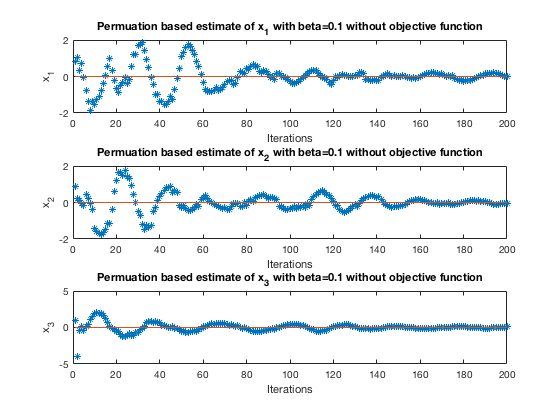
\includegraphics[width=1.1\textwidth, height=0.3\textheight]{Problem7_5.png}
    \end{minipage}%
    \begin{minipage}{0.5\textwidth}
        \centering
        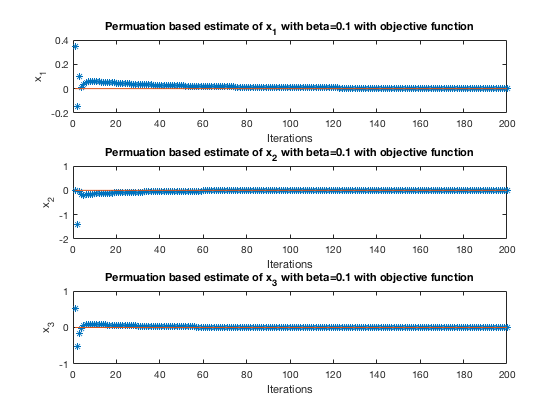
\includegraphics[width=1.1\textwidth, height=0.3\textheight]{Problem7_6.png}
    \end{minipage}
    \label{p01}
\end{figure}


\begin{figure}[H]
    \centering
    \caption{Permutation Based Convergence of $x$ for fixed value of $\beta=1$.}
    \begin{minipage}{.5\textwidth}
        \centering
        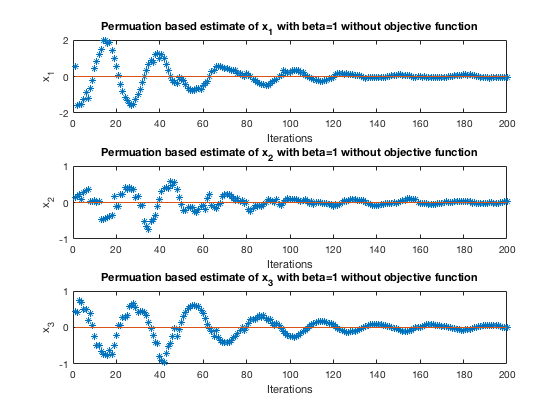
\includegraphics[width=1.1\textwidth, height=0.3\textheight]{Problem7_7.png}
    \end{minipage}%
    \begin{minipage}{0.5\textwidth}
        \centering
        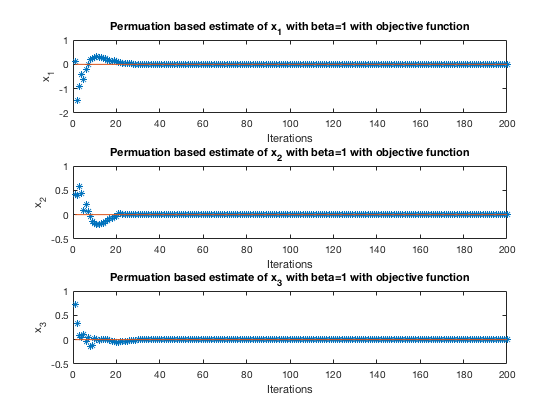
\includegraphics[width=1.1\textwidth, height=0.3\textheight]{Problem7_8.png}
    \end{minipage}
    \label{p1}
\end{figure}


\begin{figure}[H]
    \centering
    \caption{Permutation Based Convergence of $x$ for fixed value of $\beta=10$.}
    \begin{minipage}{.5\textwidth}
        \centering
        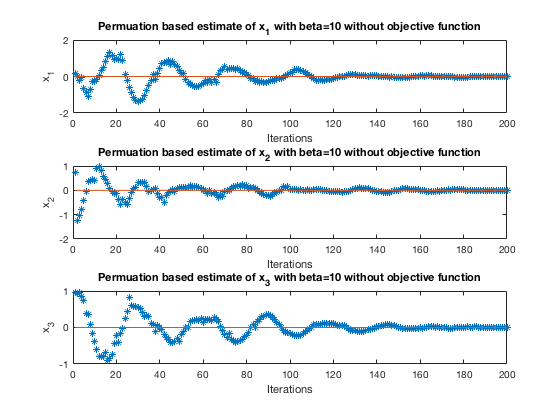
\includegraphics[width=1.1\textwidth, height=0.3\textheight]{Problem7_111.png}
    \end{minipage}%
    \begin{minipage}{0.5\textwidth}
        \centering
        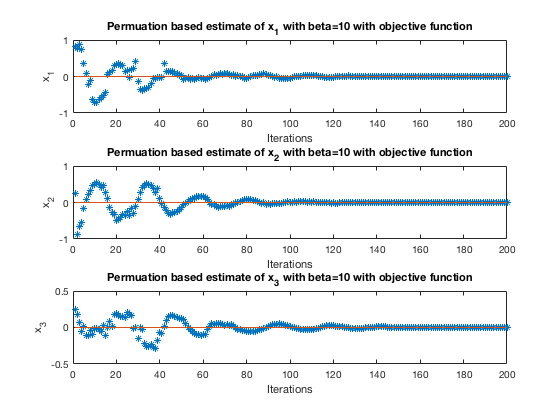
\includegraphics[width=1.1\textwidth, height=0.3\textheight]{Problem7_112.png}
    \end{minipage}
    \label{p10}
\end{figure}


 
\begin{figure}[H]
    \centering
    \caption{Permutation Based $||Ax||$ for all Methods.}
    \begin{minipage}{.5\textwidth}
        \centering
        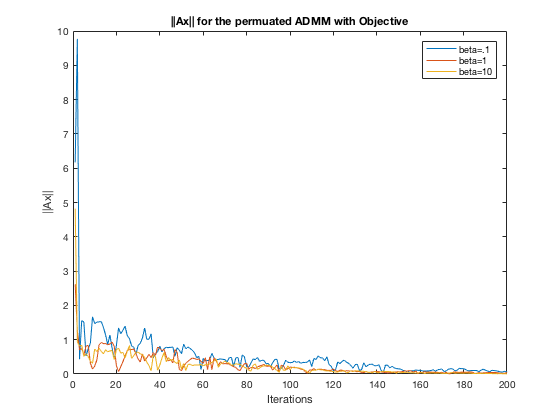
\includegraphics[width=1.1\textwidth, height=0.3\textheight]{Problem7_113a.png}
    \end{minipage}%
    \begin{minipage}{0.5\textwidth}
        \centering
        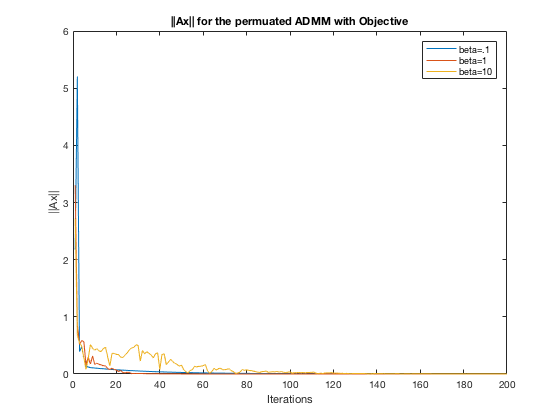
\includegraphics[width=1.1\textwidth, height=0.3\textheight]{Problem7_114a.png}
    \end{minipage}
    \label{normperm}
\end{figure}

Fig.~\ref{normperm} shows the norm of the product of a matrix $A$  and a solution of the problem $x$. As it can be easily seen from the plot, the ADMM with permutation successfully finds the optimal solution and thus the norm converges to 0 (as the solution of the problem is $x=0$). The only difference in the we notice is the periodic behavior of the convergence and the speed with which the method attains the lower bound for different value of $\beta$. As previously discussed, the fastest convergence is associated with the largest value of $\beta$ when the objective function is present in the original problem and the smallest $\beta$ when the objective is absent from the formulation.
~\\


\end{framed}
\end{itemize}

\newpage

\subsection*{Problem 8}
All pieces of Computation Team Work stated above, and one more described below.

You understand the SDP relaxation for SNL very well now, e.g., the two sensors and three anchors formulation: Find
\[Z=\left(\begin{array}{cc}
              I & X\\
              X^T& Y\end{array}\right)\in S^4
\]
to meet the constraints in the standard form:
\[\begin{array}{cl}
(1;0;0;0)(1;0;0;0)^T\bullet Z &=1,\\
(0;1;0;0)(0;1;0;0)^T\bullet Z& =1,\\
(1;1;0;0)(1;1;0;0)^T\bullet Z& =2,\\
(a_i;-1;0)(a_i;-1;0)^T\bullet Z &= d^2_{1i},\ i=1,2,\\
(a_i;0;-1)(a_i;0;-1)^T\bullet Z &= d^2_{2i},\ i=2,3,\\
(0;0;1;-1)(0;0;1;-1)^T\bullet Z&=\hat{d}^2_{12},\\
Z &\succeq 0\in S^4.
\end{array}
\]
where no objective function is present. 

The question is: could we add an suitable (or regulative) objective function to improve localization quality:
\[\begin{array}{ccl}
\min          &  C\bullet Z &\\
\mbox{s.t.}&(1;0;0;0)(1;0;0;0)^T\bullet Z &=1,\\
&(0;1;0;0)(0;1;0;0)^T\bullet Z& =1,\\
&(1;1;0;0)(1;1;0;0)^T\bullet Z& =2,\\
&(a_i;-1;0)(a_i;-1;0)^T\bullet Z &= d^2_{1i},\ i=1,2,\\
&(a_i;0;-1)(a_i;0;-1)^T\bullet Z &= d^2_{2i},\ i=2,3,\\
&(0;0;1;-1)(0;0;1;-1)^T\bullet Z&=\hat{d}^2_{12},\\
&Z &\succeq 0\in S^4.
\end{array}
\]
Try the following regulative objectives and construct the corresponding objective matrix $C$, and see which works best:

\begin{enumerate}[topsep=0pt,itemsep=-1ex,partopsep=1ex,parsep=1ex]
    


\item Minimize the trace of $Z$
\item Maximize the trace of $Z$,
\item Minimize the sum of all the non-edge distance squares (a non-edge is a edge whose distance information is unknown)
\item Maximize the sum of the non-edge distance squares
\end{enumerate}
\rule{\textwidth}{1pt}
\subsubsection*{Solution}
\newpage




    \begin{figure}[H]
    \centering
    
    \caption{Log Error of All Methods for 900 Iterations when x is Fixed at (1, 0)}
    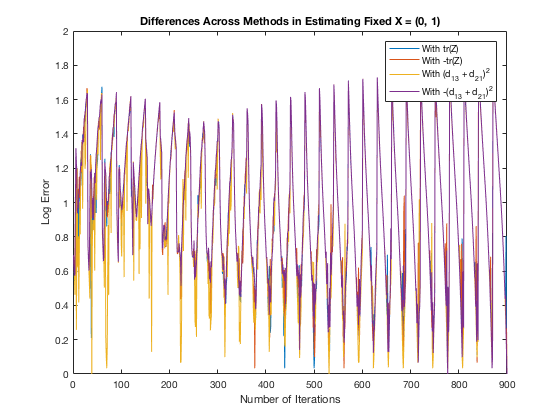
\includegraphics[width=\linewidth, height = 10cm]{Problem8harmc.png}
    \label{le900c}
    \caption{Log Error of All Methods for the First 49 Iterations when x is Fixed at (1, 0)}
    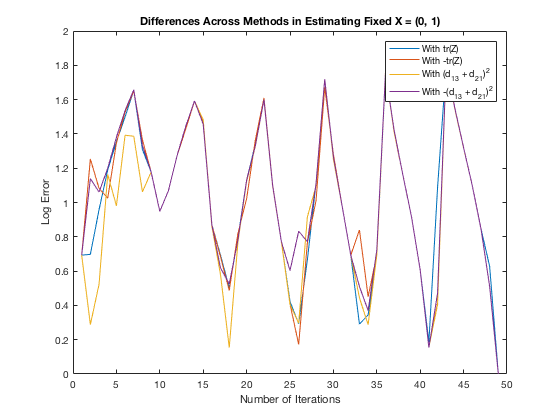
\includegraphics[width=\linewidth, height = 10cm]{Problem8prioc.png}
    \label{le49c}
    \end{figure} 
    

    
    
    
    \begin{figure}[H]
     \centering
        \caption{Log Error of All Methods for 900 Iterations when x is Fixed at (0.75, 0.35)}
    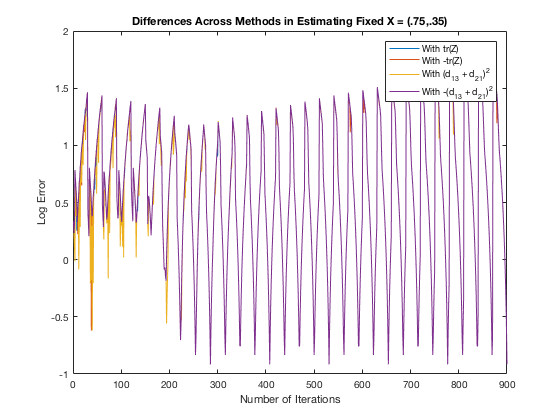
\includegraphics[scale=.65]{Problem8harmvf.png}
    \label{le900v}
    \end{figure}
    
    
    \begin{figure}[H]
    \centering
    
        \caption{Log Error of All Methods for the First 49 Iterations when x is Fixed at (0.75, 0.35)}
    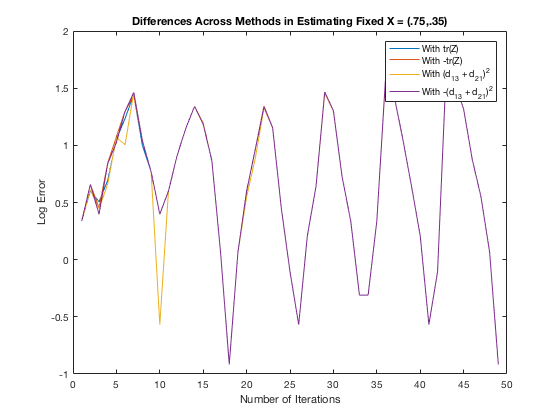
\includegraphics[scale=.65]{Problem8priov.png}
    \label{le49v}
    \end{figure}
    
    From plots depicted in Fig.~\ref{le900c}-\ref{le49v}, it can be noticed that the smallest magnitude of the error in estimating x is associated with method that uses a minimization of the sum of all non-edge distance squared as a regularizer. It should also be noted that a regularizer that minimizes the trace of Z performs well across all 900 iterations (Fig.~16 and Fig.~18), however it has bigger magnitude of error than the method mentioned above. Also, we notice that the magnitude of the error is mostly the same across methods when $x$ is fixed at (0.75, 0.35). The explanation behind this phenomena is simple. When $x$ is fixed closed to a vertex, each one of the given methods has a problem with finding an accurate value of $x$.
    
 
    
    
    
        \begin{figure}[H]
    \centering
    \caption{Histogram of the Log Error for Each Method for the first 900 Iterations when $x$ is fixed at (0,1) and (0.75, 0.35)}
    \begin{minipage}{.5\textwidth}
        \centering
        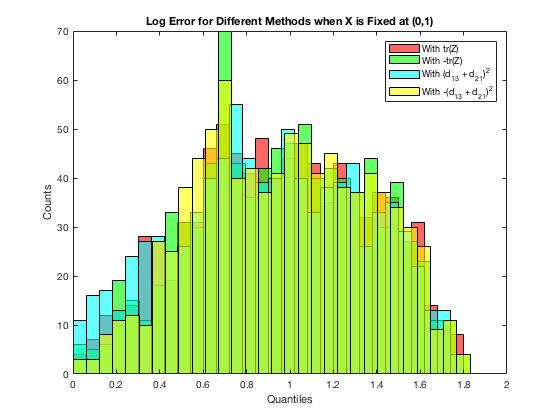
\includegraphics[width=1.1\textwidth, height=0.3\textheight]{Problem8hcf.png}
    \end{minipage}%
    \begin{minipage}{0.5\textwidth}
        \centering
        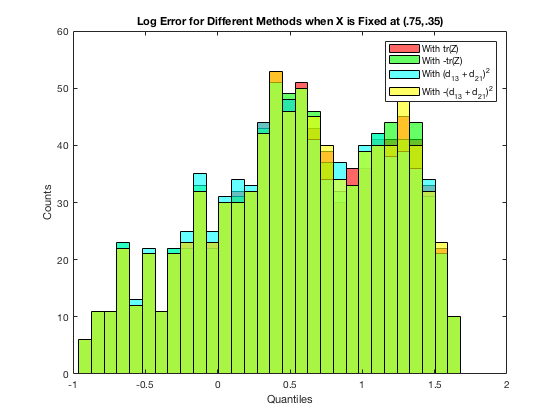
\includegraphics[width=1.1\textwidth, height=0.3\textheight]{Problem8hvf.png}
    \end{minipage}
    \label{fhist}
\end{figure}
    
    
    
    
    \begin{figure}[H]
    \centering
    \caption{Histogram of the Log Error for Each Method for the first 200 Iterations}
    \begin{minipage}{.5\textwidth}
        \centering
        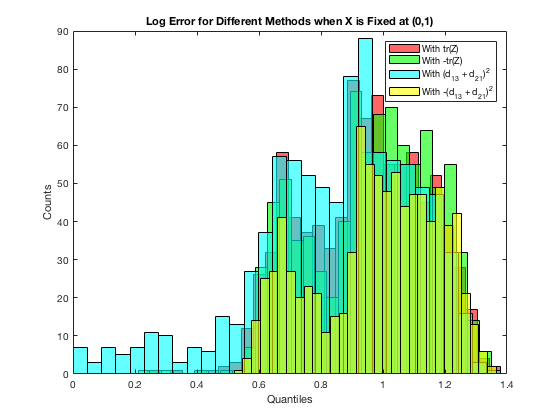
\includegraphics[width=1.1\textwidth, height=0.25\textheight]{Problem8hc.png}
    \end{minipage}%
    \begin{minipage}{0.5\textwidth}
        \centering
        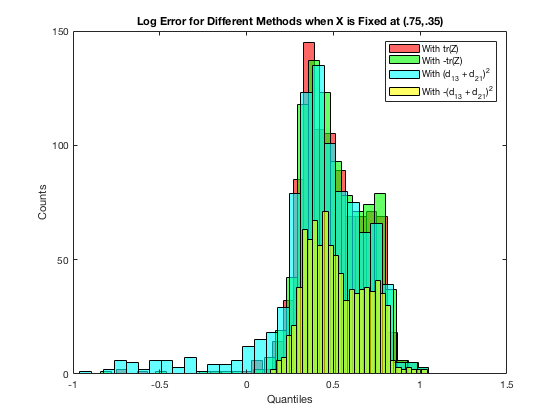
\includegraphics[width=1.1\textwidth, height=0.25\textheight]{Problem8hv.png}
    \end{minipage}
    \label{phist}
\end{figure}
    
    
     Similarly to the previously stated argument, we observe that histograms depicted by Fig.~\ref{fhist} and Fig.~\ref{phist} show that the the method that uses the minimization of the sum of all non-edge distance squared has the smallest magnitude of error for almost all 900 different points (iterations), similarly for only first 200 estimations. It should also be noted that when $x$ is fixed at $(0.75, 0.35)$ the overall difference in the magnitude of the error is smaller across all the methods when the number of points that we try to find is large. That is, all methods have similar error when estimating the value of $x$. 
    
    
        \begin{figure}[H]
    \centering
    
        \caption{Magnitude of Error when X is Fixed at (0,1) and the Objective is to Minimize the Trace of Z.}
    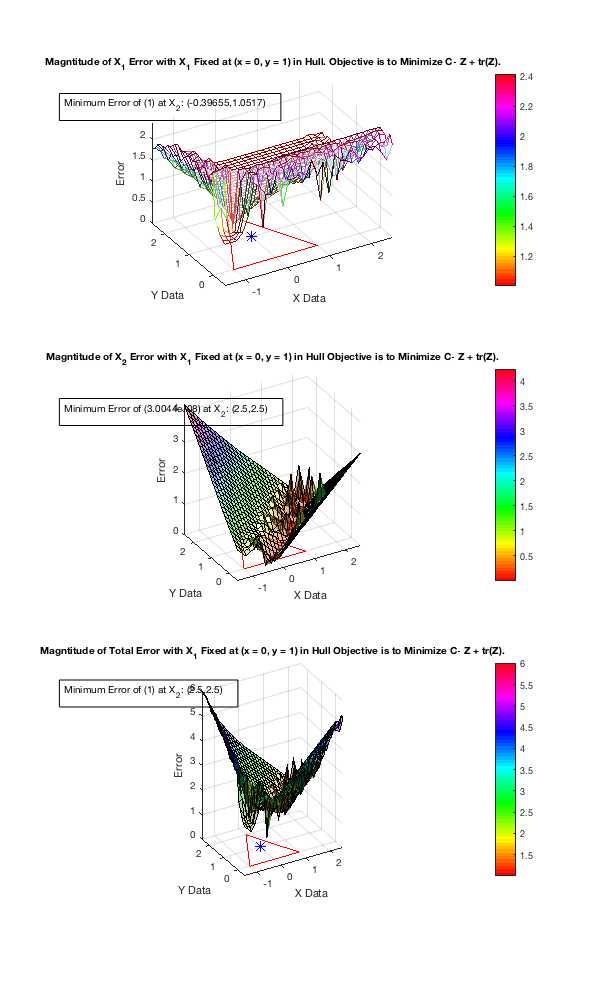
\includegraphics[scale=.7]{Problem8f1.png}
    \end{figure} 
    
        \begin{figure}[H]
    \centering
    
        \caption{Magnitude of Error when X is Fixed at (0.75,0.35) and the Objective is to Minimize the Trace of Z.}
    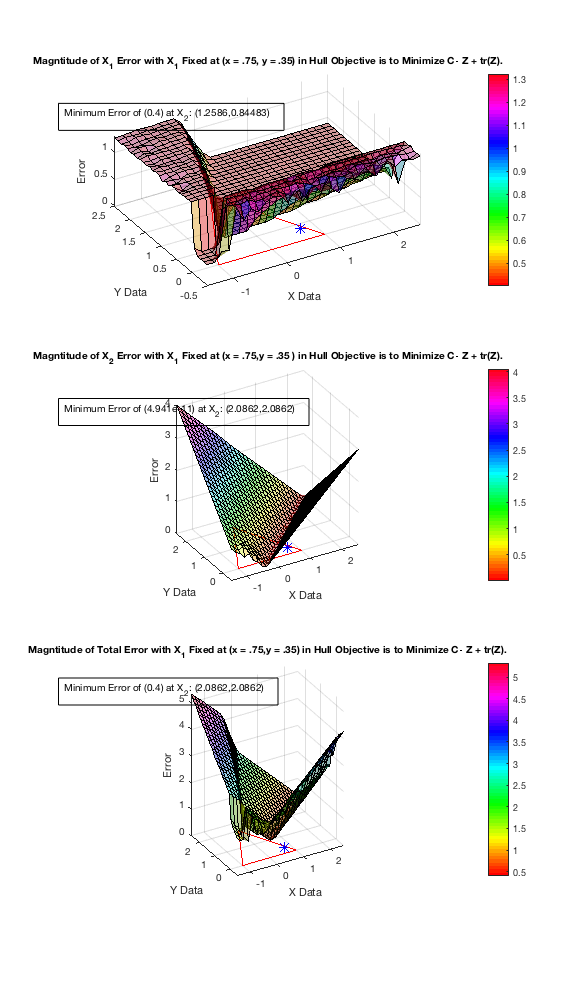
\includegraphics[scale=.7]{Problem8f2.png}
    \end{figure} 
    
        \begin{figure}[H]
    \centering
    
        \caption{Magnitude of Error when X is Fixed at (1,0) and the Objective is to Maximize the Trace of Z.}
    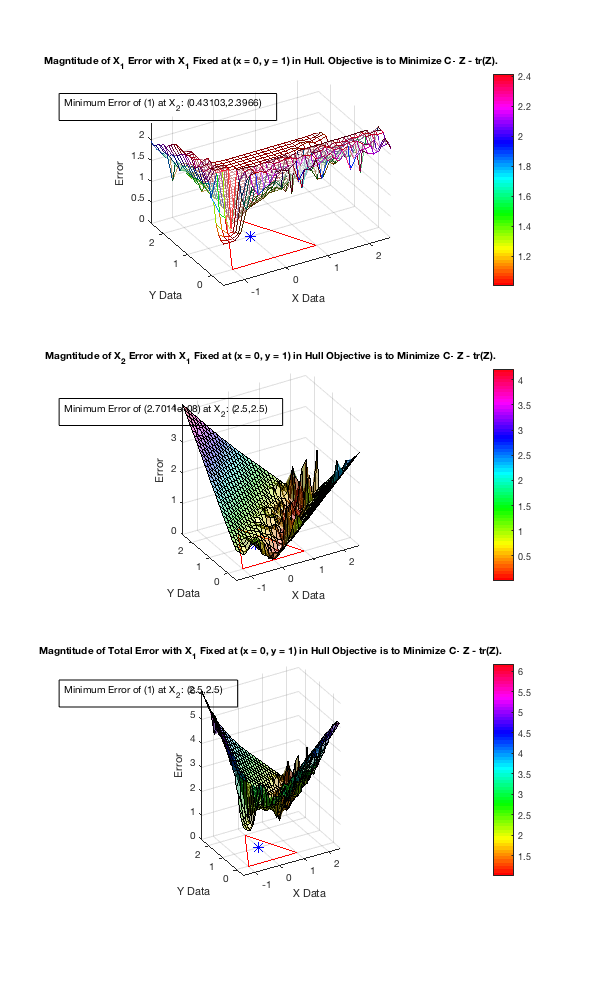
\includegraphics[scale=.7]{Problem8f3.png}
    \end{figure} 
    
        \begin{figure}[H]
    \centering
    
        \caption{Magnitude of Error when X is Fixed at (.75,.35) and the Objective is to Maximize the Trace of Z.}
    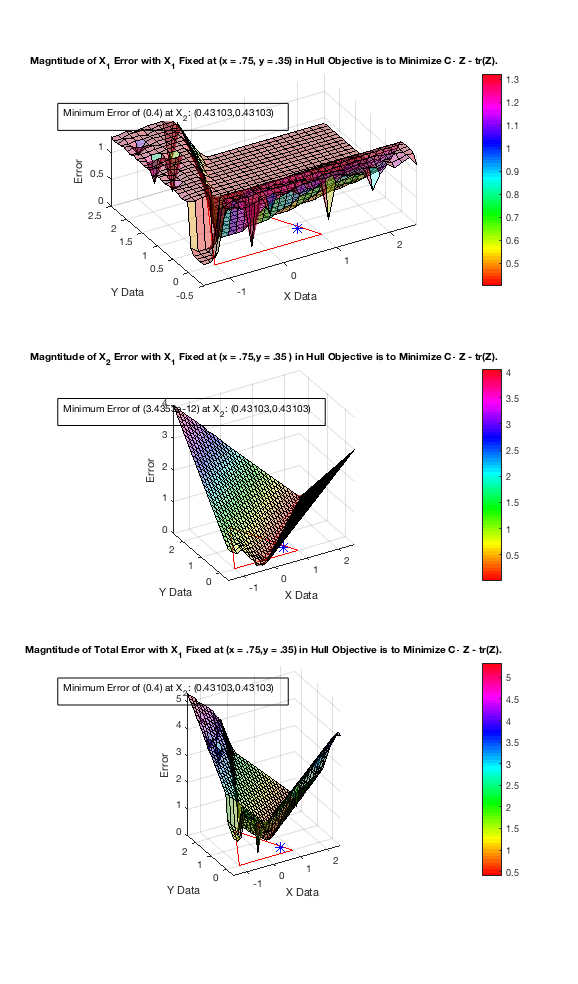
\includegraphics[scale=.7]{Problem8f4.png}
    \end{figure} 
    
        \begin{figure}[H]
    \centering
    
        \caption{Magnitude of Error when X is Fixed at (1,0) and the Objective is to Minimize the Distance.}
    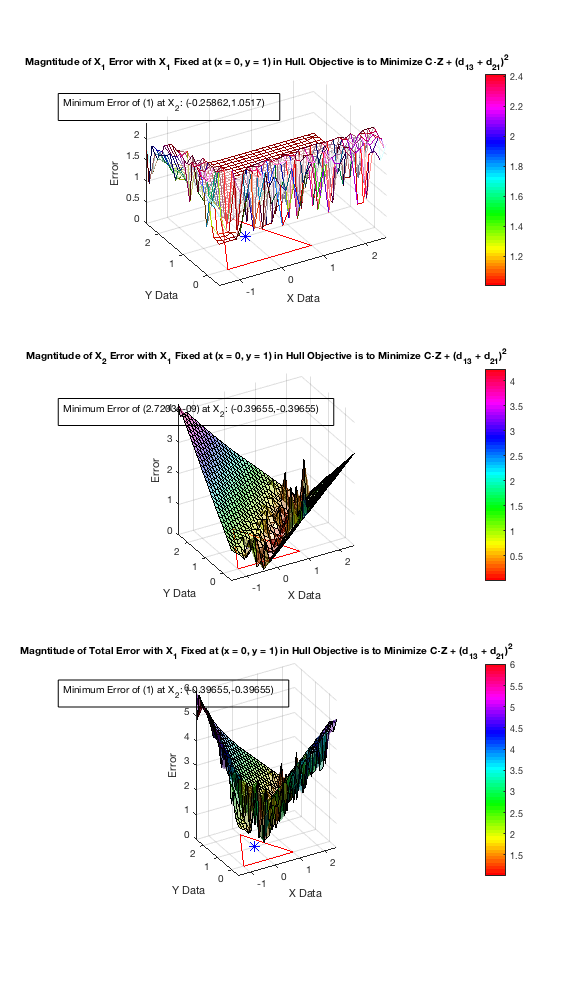
\includegraphics[scale=.7]{Problem8f5.png}
    \end{figure} 
    
        \begin{figure}[H]
    \centering
    
        \caption{Magnitude of Error when X is Fixed at (.75,.35) and the Objective is to Minimize the Distance.}
    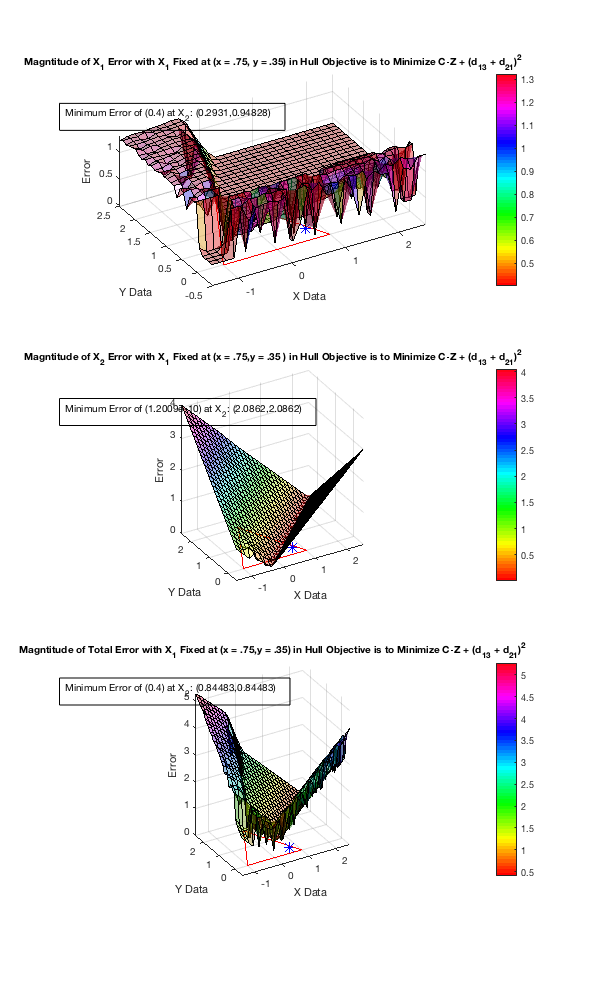
\includegraphics[scale=.7]{Problem8f6.png}
    \end{figure} 


  \begin{figure}[H]
    \centering
    
        \caption{Magnitude of Error when X is Fixed at (0,1) and the Objective is to Maximize the Distance.}
    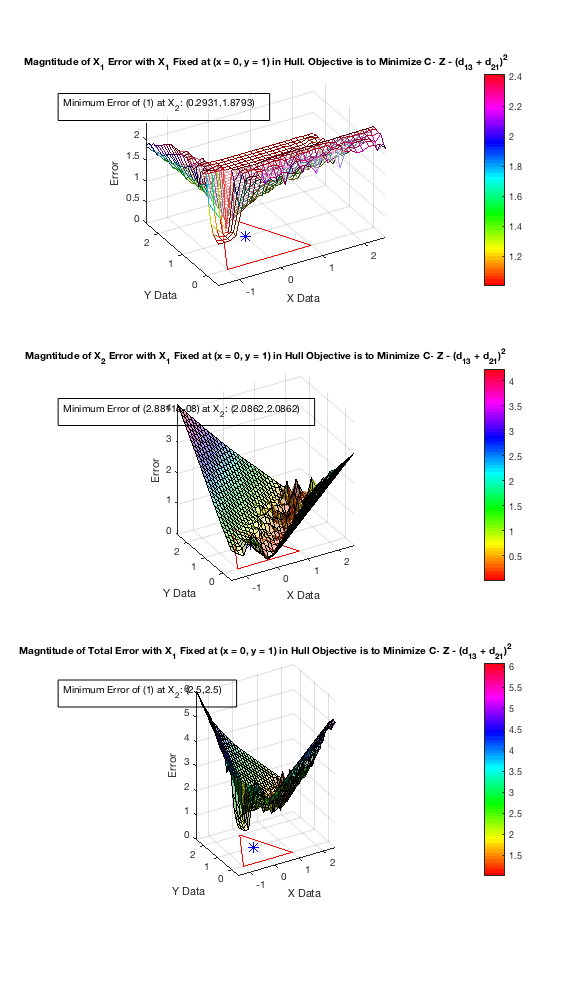
\includegraphics[scale=.7]{Problem8f7.png}
    \end{figure} 
    
        \begin{figure}[H]
    \centering
    
        \caption{Magnitude of Error when X is Fixed at (0.75,0.35) and the Objective is to Maximize the Distance.}
    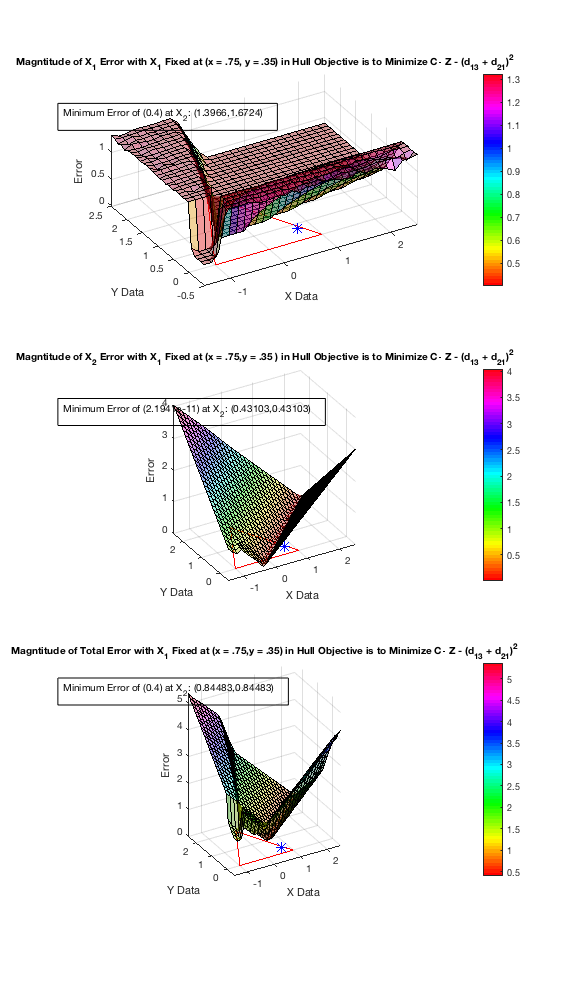
\includegraphics[scale=.7]{Problem8f8.png}
    \end{figure} 
    
    \rule{\textwidth}{1pt}

\end{document}